\chapter{State of the art}

The laws governing the processes of heat transfer and fluid flow are usually expressed in terms of differential equations. These equations are the momentum equation, the energy equation and the mass conservation equation, among others. However, these expressions don’t have an analytical solution except for some simple cases. To solve complex problems it is necessary to use numerical methods.

\section{Conservation equations}
\label{ConservationEquations}
The three most important conservation equations are the mass conservation equation, the momentum conservation equation and the energy conservation equation:
\begin{equation}
\frac{\partial\rho}{\partial t}+\nabla\cdot\left(\rho\vec{v}\right)=0
\end{equation}
\begin{equation}
\frac{\partial}{\partial t}\left(\rho\vec{v}\right)+\nabla\cdot\left(\rho\vec{v}\vec{v}\right)=-\nabla p+\nabla\cdot\vec{\tau}+\rho\vec{g}+\vec{f^{e}}
\end{equation}
\begin{equation}
\frac{\partial}{\partial t}(\rho u)+\nabla\cdot\left(\rho\vec{v}u\right)=-\nabla\cdot\vec{\dot{q}}-p\nabla\cdot\vec{v}+\vec{\tau}:\nabla\vec{v}+\Phi^{e}
\end{equation}

These equations can be simplified depending on the case that is being studied. For example, for incompressible flows with no viscous dissipation, the energy conservation equation can be written as:
\begin{equation}
\rho c_{p}\left(\frac{\partial T}{\partial t}+\vec{v}\cdot\nabla T\right)=\nabla\cdot\left(\lambda\nabla T\right)
\label{EnergyIncompNoVisc}
\end{equation}

All these equations can be seen as a particular case of the generic convection-diffusion equation:
\begin{equation}
\frac{\partial}{\partial t}\left(\rho\phi\right)+\nabla\cdot\left(\rho\vec{v}\phi\right)=\nabla\cdot\left(\Gamma\nabla\phi\right)+S_{\phi}
\end{equation}
where $\rho$ is the density, $\vec{v}$ the velocity, $\Gamma$ the diffusion coefficient, $S_{\phi}$ the source term, and $\phi$ the general variable that is going to be studied. Table \ref{convdifeq} lists the values that these variables have to take in order to obtain the conservation equations previously mentioned.

\begin{table}[h!]
	\centering
	\begin{tabular}{ |c|c|c|c| } 
		\hline
		Equation & $\phi$ & $\Gamma$ & $S_{\phi}$ \\ \hline 
		Mass conservation & $1$ & $0$ & $0$ \\  \hline
		Momentum & $\vec{v}$ & $\mu$ & $-\nabla p+\nabla\cdot\vec{\tau}+\rho\vec{g}+\vec{f^{e}}$ \\  \hline
		Energy (for a semiperfect gas) & $u$ & $\lambda/c_{v}$ & $-\nabla\cdot\vec{\dot{q}}-p\nabla\cdot\vec{v}+\vec{\tau}:\nabla\vec{v}+\Phi^{e}$ \\
		\hline
	\end{tabular}
\caption{Particular cases of the convection-diffusion equation}
\label{convdifeq}
\end{table}

\section{Numerical methods}
Numerical methods are based in dividing the domain that is going to be studied in different pieces. Instead of calculating the unknowns in the whole domain, they are studied in the finite number of points defined by these pieces: the grid points. This process is called discretization.

Once the domain is discretized, it is also necessary to discretize the equations. The relations between the grid points have to be established. It is assumed that the value $\phi$ of a grid point only influences the distribution of $\phi$ in its immediate neighbours. Consequently, as the number of grid points becomes larger, the numerical solution approaches the real solution of the problem.

\section{Finite difference method}
The finite difference method (FDM) is a discretization method based in the Taylor-series expansion. It is used to approximate the derivatives in the differential equation. Taking the three successive points represented in figure \ref{3gridpoints}, the approximation of the values in the left point (west) and in the right point (east) is easily calculated with Taylor series:
\begin{equation}
\phi_{W}=\phi_{P}-\Delta x\left(\frac{d\phi}{dx}\right)_{P}+\frac{1}{2}\left(\Delta x\right)^{2}\left(\frac{d^{2}\phi}{dx^{2}}\right)-\dots
\end{equation}
\begin{equation}
\phi_{E}=\phi_{P}+\Delta x\left(\frac{d\phi}{dx}\right)_{P}+\frac{1}{2}\left(\Delta x\right)^{2}\left(\frac{d^{2}\phi}{dx^{2}}\right)+\dots
\end{equation}
Using a second order approximation and combining both expressions:
\begin{equation}
\left(\frac{d\phi}{dx}\right)_{P}\approx\frac{\phi_{E}-\phi_{W}}{2\Delta x}
\end{equation}
\begin{equation}
\left(\frac{d^{2}\phi}{dx^{2}}\right)_{P}\approx\frac{\phi_{W}+\phi_{E}-2\phi_{P}}{\left(\Delta x\right)^{2}}
\end{equation}
These expressions are substituted in the differential equation to obtain the finite-differential equation. This approach is very simple, but it is not used in complex geometries. It also does not enforce conservation, as it is simply a mathematical approach.
\begin{figure}
	\centering
	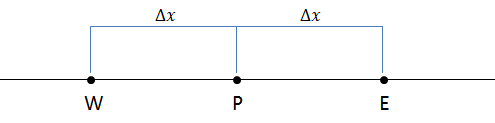
\includegraphics[scale=0.8]{StateArt/3gridpoints}
	\caption{Three successive grid points}
	\label{3gridpoints}
\end{figure}

\section{Finite volume method}
The finite-volume method (FVM) is another discretization method more used than the FDM. It consists in dividing the domain in different control volumes as the ones in figure \ref{controlvolume2d}, so that each control volume surrounds one grid point. The differential equation is integrated over each control volume, ensuring that each of them satisfies the conservation principle. It is the method used in the present study.
\begin{figure}[h!]
	\centering
	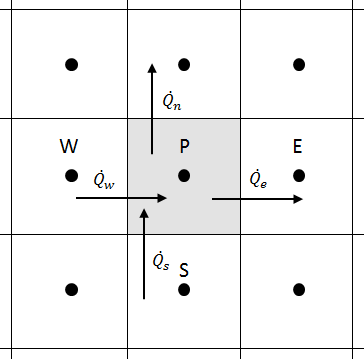
\includegraphics[scale=0.5]{StateArt/controlvolume2d}
	\caption{Control volume (2D)}
	\label{controlvolume2d}
\end{figure}

\subsection{Mesh}
There are different ways to discretize the domain for the FVM. Some of these methods are listed below \cite{Ferziger2002}:
\begin{itemize}
	\item Structured (regular) mesh: Grid lines do not cross each other. Lines can be numbered consecutively, so that the position of any grid point can be easily identified by two (2D) or three (3D) indices. It is equivalent to a Cartesian grid. This is the simplest structure and easiest to work with, but it can only be used for geometrically simple domains.
	\item Unstructured mesh: The control volumes may have any shape, and there is not a restriction on the number of neighbour nodes. It is the method used for very complex geometries, but the grid generation and the pre-processing are more difficult than on structured meshes.
\end{itemize}

\section{Time integration}
Time is a one-way variable, which means that the unknowns only depend on the values in the previous instant of time, and do not depend on the values in the next instant of time. Knowing this property, to obtain the results of an unsteady problem, it is only necessary to discretize the time domain in time steps and calculate the values in each of them. When the unknowns of one time step are obtained, the calculation moves on to the next time step.

Time integration can be done using different methods. The ones that are widely used are:
\begin{itemize}
	\item Explicit method: The simplest method. The terms are evaluated using the known values of the previous time step $t^{n}$. It is a first order approximation and easy to compute, but it requires very small time steps in order to achieve convergence.
	\item Implicit method: It is a very stable first order approximation, which makes it useful in problems with large time steps. The terms are evaluated with the values in the next instant of time $t^{n+1}$.
	\item Crank-Nicholson: It is a second order approximation. The terms are evaluated using the values of the previous and the next time step.
\end{itemize}

\section{Interpolation schemes}
In some cases, it is necessary to obtain the properties of the points that are not nodes. Some terms are evaluated in the faces, not in the nodes, so it is necessary to calculate the values of the variables in the faces of the control volume. There are different schemes to do so.  Some of the most common ones are listed below\cite{Patankar1980,Ferziger2002}.

\subsection{The central differencing scheme (CDS)}
It is the most natural scheme. It is a linear interpolation between the two nearest nodes:
\begin{equation}
\phi_{e}-\phi_{P}=\frac{d_{Pe}}{d_{PE}}\left(\phi_{E}-\phi_{P}\right)
\end{equation}
However, CDS is only valid in cases with low Reynolds number. It is a second order approximation, but may produce oscillatory solutions.

\subsection{The upwind scheme (UDS)}
It assumes that the value of $\phi$ in the interface is equal to the value of $\phi$ at the node on the upwind side of the face:
\begin{equation}
\begin{aligned}
\phi_ {e} &=\phi_{P},&&\text{if $\dot{m}_{e}>0$}\\    \phi_ {e} &=\phi_{E},&&\text{if $\dot{m}_{e}<0$}
\end{aligned}
\end{equation}
The solutions of the UDS are always physically realistic, but they may not be completely accurate because it is a first order approximation. However, this method is widely used due to its stability.

\subsection{The exponential scheme (EDS)}
Taking the generic convection-diffusion equation and assuming a steady one-dimensional problem with constant $\Gamma$ and no source term, the analytic solution of the equation is an exponential function:
\begin{equation}
\frac{\phi-\phi_{0}}{\phi_{L}-\phi_{0}}=\frac{exp\left(Px/L\right)-1}{exp\left(P\right)-1}
\end{equation}
where $\phi_{0}$ and $\phi_{L}$ are the values of the function at $x=0$ and $x=L$ respectively, and P is the Péclet number, a non-dimensional number:
\begin{equation}
P\equiv\frac{\rho uL}{\Gamma}
\end{equation}
In the EDS, this analytic solution is used to determine the value on the faces, using the following expression:
\begin{equation}
\phi_{e}-\phi_{P}=\frac{exp\left(P_{e}d_{Pe}/d_{PE}\right)-1}{exp\left(P_{e}\right)-1}\left(\phi_{E}-\phi_{P}\right)
\end{equation}
Though this solution is exact for the steady one-dimensional problem it is not for two or three-dimensional cases, unsteady problems and cases with source term, so it is not widely used.

\subsection{The hybrid scheme (HDS) and the power-law scheme (PLDS)}
Both methods are an approximation of the exponential function used in the EDS. Since exponentials are expensive to compute, the HDS and the PLDS are meant to provide a good result but with simpler functions. They divide the function given by the EDS in different parts and approximate the solution with simpler functions \cite{Patankar1980}.